% This is the Reed College LaTeX thesis template. Most of the work
% for the document class was done by Sam Noble (SN), as well as this
% template. Later comments etc. by Ben Salzberg (BTS). Additional
% restructuring and APA support by Jess Youngberg (JY).
% Your comments and suggestions are more than welcome; please email
% them to cus@reed.edu
%
% See http://web.reed.edu/cis/help/latex.html for help. There are a
% great bunch of help pages there, with notes on
% getting started, bibtex, etc. Go there and read it if you're not
% already familiar with LaTeX.
%
% Any line that starts with a percent symbol is a comment.
% They won't show up in the document, and are useful for notes
% to yourself and explaining commands.
% Commenting also removes a line from the document;
% very handy for troubleshooting problems. -BTS

% As far as I know, this follows the requirements laid out in
% the 2002-2003 Senior Handbook. Ask a librarian to check the
% document before binding. -SN

%%
%% Preamble
%%
% \documentclass{<something>} must begin each LaTeX document
\documentclass[12pt,twoside]{reedthesis}
% Packages are extensions to the basic LaTeX functions. Whatever you
% want to typeset, there is probably a package out there for it.
% Chemistry (chemtex), screenplays, you name it.
% Check out CTAN to see: http://www.ctan.org/
%%
\usepackage{graphicx,latexsym}
\usepackage{amssymb,amsthm,amsmath}
\usepackage{longtable,booktabs,setspace}
\usepackage{chemarr} %% Useful for one reaction arrow, useless if you're not a chem major
\usepackage[hyphens]{url}
\usepackage{rotating}
\usepackage{natbib}
\usepackage{todonotes}
\usepackage{hyperref}
\usepackage{verbatim}
\usepackage{epigraph}
\usepackage{lmodern}

%% Added for comments
\usepackage{color}
\newcommand{\anna}[1]{{\color{blue}[AR: #1]}}
\theoremstyle{definition}
\newtheorem{definition}{Definition}[section]

%% Preface quote stuff
\newlength\longest

%% Graphics path
\graphicspath{ {figures/} }

% Comment out the natbib line above and uncomment the following two lines to use the new
% biblatex-chicago style, for Chicago A. Also make some changes at the end where the
% bibliography is included.
%\usepackage{biblatex-chicago}
%\bibliography{thesis}

\newcommand{\argmax}{\arg\!\max}

% \usepackage{times} % other fonts are available like times, bookman, charter, palatino

\title{Prize-Collecting Steiner Trees in Directeded Signaling Hypergraphs}
\author{Barney Isaksen Potter}
% The month and year that you submit your FINAL draft TO THE LIBRARY (May or December)
\date{May 2016}


%\division{Mathematics and Natural Sciences}
\advisor{Dr. Anna Ritz}
%If you have two advisors for some reason, you can use the following
\altadvisor{Dr. James Fix}
%%% Remember to use the correct department!
\department{Interdisciplinary Committee for Mathematics \& Biology}
% if you're writing a thesis in an interdisciplinary major,
% uncomment the line below and change the text as appropriate.
% check the Senior Handbook if unsure.
\thedivisionof{The Division of Mathematics \& Natural Sciences}
% if you want the approval page to say "Approved for the Committee",
% uncomment the next line
\approvedforthe{Committee}

\setlength{\parskip}{0pt}
%%
%% End Preamble
%%
%% The fun begins:
\begin{document}

  \maketitle
  \frontmatter % this stuff will be roman-numbered
  \pagestyle{empty} % this removes page numbers from the frontmatter

% Acknowledgements (Acceptable American spelling) are optional
% So are Acknowledgments (proper English spelling)
    \chapter*{Acknowledgments}
	I want to thank a few people:

  \begin{itemize}
    \item{Mom and Dad}
    \item{Mari}
    \item{Far Far}
    \item{Sam, Will, Rich, and ext. family}
    \item{Helen and Melvin}
    \item{Michael and Caleb}
    \item{Anna and Jim}
    \item{Sarah, Jeremy, Leigh, and the Schaack Lab}
    \item{My benefactor}
    \item{A.T \& A.L} %Turing and Lovelace
  \end{itemize}

% The preface is optional
% To remove it, comment it out or delete it.
    \chapter*{Preface}
	%\epigraph{We can only see a short distance ahead, but we can see plenty there that needs to be done.}{\textit{Alan Turing}}
  \null\vfill

\settowidth\longest{\huge\itshape just as his inclination leads him;}
\begin{center}
\parbox{\longest}{%
  \raggedright{\huge\itshape%
   We can only see \\
  a short distance ahead, \\
  but we can see plenty there \\
  that needs to be done.\par\bigskip
  }
  \raggedleft\Large\MakeUppercase{Alan Turing}\par%
}
\end{center}

\vfill\vfill


    \tableofcontents
% if you want a list of tables, optional
    \listoftables
% if you want a list of figures, also optional
    \listoffigures

% The abstract is not required if you're writing a creative thesis (but aren't they all?)
% If your abstract is longer than a page, there may be a formatting issue.
    \chapter*{Abstract}
	The preface pretty much says it all.

	\chapter*{Dedication}
	You can have a dedication here if you wish.

  \mainmatter % here the regular arabic numbering starts
  \pagestyle{fancyplain} % turns page numbering back on

%The \introduction command is provided as a convenience.
%if you want special chapter formatting, you'll probably want to avoid using it altogether

    \chapter*{Introduction}
         \addcontentsline{toc}{chapter}{Introduction}
	\chaptermark{Introduction}
	\markboth{Introduction}{Introduction}
	% The three lines above are to make sure that the headers are right, that the intro gets included in the table of contents, and that it doesn't get numbered 1 so that chapter one is 1.

% Double spacing: if you want to double space, or one and a half
% space, uncomment one of the following lines. You can go back to
% single spacing with the \singlespacing command.
\onehalfspacing
% \doublespacing

Since the discovery of cells by Robert Hooke in 1665, biologists have worked tirelessly to unlock the mysteries of cell function. Over the last half-century, our knowledge of how cells function has grown tremendously. An important and growing part of this field has been the

 \section{Network Representations}

 \section{Graph Theory}

 \section{The Steiner Tree Problem}

  \subsection{Prize-Collecting Steiner Tree Problem}

 \section{Integer Linear Programming}

\chapter{Cell Signaling Networks}

Cell function is governed by countless interactions between proteins, nucleic acids, lipids, carbohydrates, and many other small molecules.  The interactions between all of these components form what we call \textit{cell signaling networks}, which are responsible for almost every process within a cell.  Cell signaling networks are used to describe how many of the most basic reactions within cells cause propagations of information, and the results of thse signals.  Some of the most important types of interactions that we see in cell signaling networks (also refered to as protein-protein interaction or signal transduction networks) include the assembly and destruction of protein complexes, how small molecules such as ATP interact with proteins, the cascade of events that can occur after a membrane-bound protein is bound by a ligand, or where negative feedback loops exist that can have an effect on cell function.  We often refer to these cell signaling networks at protein-protein interaction (PPI) networks.  Historically, PPI networks have been a useful tool for compiling knowledge about individual interactions that have been studied \textit{in situ}, so that larger scale patterns of interaction can be examined, and both communicated easily and analyzed algorithmically. In recent years, there has been a push to find ways to accurately model these networks so that they can be used to predict potential areas of future research (CITATION), in particular, by using graph-based methods (\cite{Aittokallio2006}).\par

Generally speaking, there are a few key steps to a cell signling network. First, a trans-membrane protein will undergo a conformational change in response to a particular ligand. Typically, this signal will be some sort of messenger molecule to which the cell needs to respond. The change in conformation results in a cascade of interaction between proteins and other small molecules within the cell. Some of the changes that can result from this cascade of signaling are protein complex assembly, complex degradation, conformational changes to other proteins, phosphorylation, or dephosphorylation (among many other reactions). The ultimate result of this signaling cascade is a change in one or more transcription factors, proteins that bind to DNA, and regulate the rate of transcription of DNA to mRNA.\par

\section{PPI Databases}

In recent years, there has been a push to start curating what is already known about cell signaling, and publishing these networks online (\cite{Bauer-Mehren2009}, \cite{Cusick2009}). Many of these databases have been made available to the public, so that the data that they contain can be used collaboratively by anyone. Some of these networks are the Reactome database (\texttt{reactome.org}, \cite{Matthews2009}), NetPath (\texttt{netpath.org}, \cite{Kandasamy2010}), and SPIKE (\texttt{http://spike.cs.tau.ac.il/spike2/}, \cite{Paz2010}).\par
The purpose of signaling pathway databases is twofold: to create repositories of known interactions, so that they can be easily referred to viewed in a zooomable, searchable manner (\cite{Hu2007}), and so that researchers can take advantage of the computational tools that alerady exist to find novel areas of research from these manually-curated networks (\cite{Karlebach2008}, \cite{Battle2010}).\par

\section{Signaling by \emph{Hedgehog}}
\emph{I decided to go with Hh, because a. it is a less complicated pathway, so it is easier to discuss without leaving a ton out, and b. because it has more orthologs in A. thaliana. Also, I realized that Hh disregulations are most closely associated with the kind of skin cancer that I had.}

One example of a cell signaling pathway that has a variety of biological consequences is the \textit{Hedgehog} (Hh) signal transduction network. Hedgehog is a protein that helps regulate limb formation during early development, cell development and differentiation, and the development of neural tubes (\cite{Hiu2011})

\begin{figure}[h]
  \begin{center}
    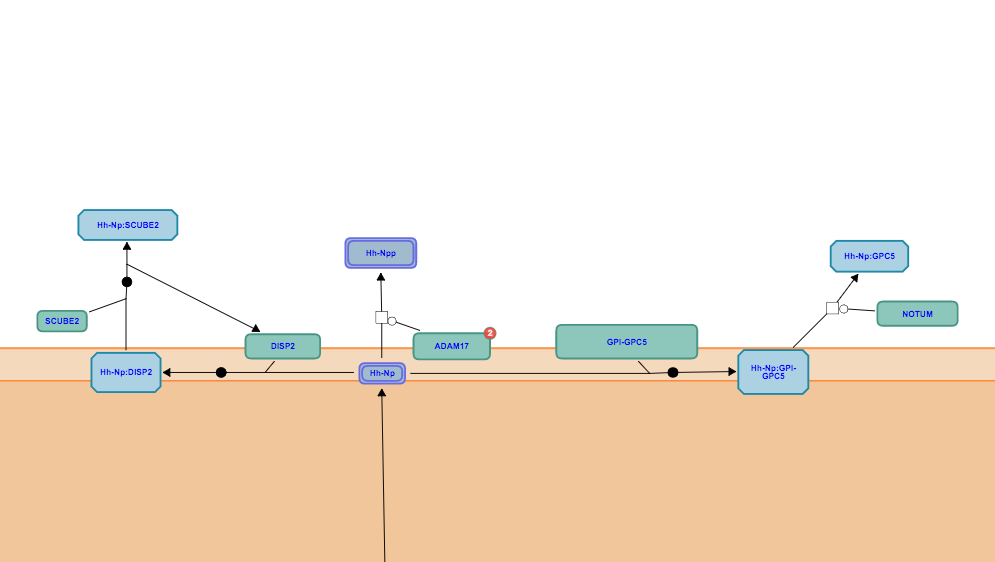
\includegraphics{Hh-Np_secretion}
  \caption{Hh-Np secretion, as shown by \texttt{reactome.org}.}
  \label{fig:Hh-Np_secretion}
  \end{center}
\end{figure}

\subsection{\emph{Hedgehog} Signaling in \emph{Homo sapiens}}

\subsection{\emph{Hedgehog} Signaling in \emph{Arabidopsis thaliana}}


\chapter{Hypergraphs \& Hyperpaths}

While standard\footnote{The term ``standard" is used to describe traditional graphs, since the terms ``regular" and ``normal," which would be natural choices, both refer to specific types of graphs.} graphs are useful for many applications, they are severely limited in their ability to represent cell-signaling interactions.  Since they can only show pairwise interactions between nodes, whenever there is an interaction that requires more than two connections, the visualization of the graph becomes confusing, and biologically meaningless.  Furthermore, interactions involving multiple molecules require an enormous amount of different edges to represent all of the sub-interactions that take place.  Determining whether two edges are part of the same biological event is a non-trivial problem, and requires manual curation to solve, at this time.\par

\begin{figure}[thbp]
  \begin{center}
    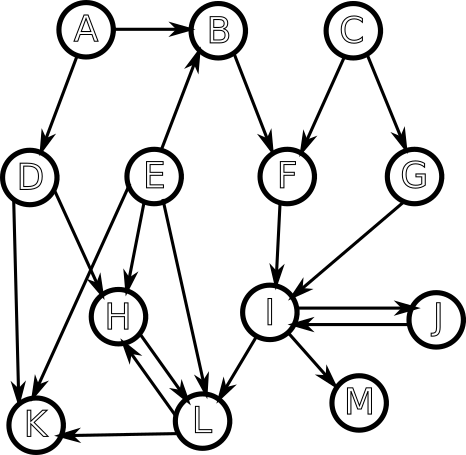
\includegraphics{example-standard-graph}
  \caption{An example of a standard graph. All edges represent directed, pairwise interactions between two nodes. Biologically, it is difficult to extract meaningful signaling pathway information from this graph, since protein complex formation and degradation is ambiguous.}
  \label{fig:example-standard-graph}
  \end{center}
\end{figure}

One area of cell-signaling that becomes particularly problematic in standard graphs is the formation, interaction, and destruction of protein complexes.  The only way that complexes can be represented in standard graphs is by creating a complete subgraph of all of the elements of the protein complex.  On their own, these complete subgraphs can yield useful information about the make-up of a protein complex, but once they begin interacting with other elements of the graph, the graph becomes much more complex, as all of the proteins in the complex must be represented independently.  In the case of interactions between multiple large complexes, it becomes the case that the standard graph representation of this interaction is a large complete subgraph that contains nodes for all of the proteins involved in either complex.  It is then computationally impossible to distinguish whether the entity being described by the subgraph is the interaction between multiple protein complexes, or simply one large complex that contains all of the components of both complexes.  Furthermore, since the complete subgraphs which represent complexes are undirected, it is extremely difficult to tell what the inputs or outputs of a biochemical reaction may be.\par

Another shortcoming of standard graphs in representing complex biological interactions is that there is no way in which to represent positive or negative regulation of interactions.  Since there is a standardized way in which edges interact with nodes, there is no way to differentiate types of interactions between nodes.  This poses a challenge when there are regulators or catalysts present that are necessary for a reaction, but are not part of the inputs or outputs of the reaction.  If regulators are to be included in a standard graph representation of a cell-signaling network, they become indistinguishable from any other types of interactions that are taking place.  This lack of specificity is problematic, as it treats all interactions as equal, and hides potentially useful information from the graph.\par

To resolve the issues presented by standard graphs, we instead use a generalization called a \textit{hypergraph} that allows for the addition of more detail  and specificity within the data structure than standard graphs allow for.  In particular, hypergraphs allow for both the representation of protein complexes in the form of \textit{hypernodes}, which we think of simply as a set of one or more nodes, and for the representation of complex, directed interactions that can have multiple inputs and outputs.  We represent these interactions with the use of \textit{hyperedges}, which define a set of one or more hypernodes.  Since a hyperedge may include more than two hypernodes, we gain the ability to represent both multi-protein interactions, as well as to define the notions of regulation on reactions.\par

\section{Prize-Collecting Steiner Hypertrees}

Where a directed graph represents directed, pairwise interactions between only two vertices, we can use \textit{directed hypergraph} to represent directed interactions between sets of vertices (nodes). We formally define a directed hypergraph, $\mathcal{H}$, as a pair $(V,E)$, where $V$ is a finite set of vertices and $E \subseteq 2^V \times 2^V$ is a finite set of \textit{directed hyperedges} connecting members of $V$ such that, for every $e=(T(e),H(e)) \in E$, $T(e) \cap H(e) = \emptyset$, and $T(e)$, $H(e) \neq \emptyset$.  We refer to $T(e)$ as the \textit{tail} of the hyperedge, and to $H(e)$ as the \textit{head} of the hyperedge.\par

Furthermore, we can define sets of two or more nodes as a hypernode, which are members of the power set of $V$.  These can be incorporated into a directed hypergraph to form a \textit{complexed directed hypergraph}.  We define a \textit{complexed directed hypergraph}, $\mathcal{H}$, as the triple $(V,U,E)$ in which $V$ is a finite set of vertices, $U \subseteq 2^V$ is a finite set of hypernodes, and $E \subseteq 2^U \times 2^U$ is a finite set of hyperedges such that, for every $e=(T(e),H(e)) \in E$, $T(e) \cap H(e) = \emptyset$ and $T(e)$, $H(e) \neq \emptyset$.\par

\begin{figure}[thbp]
  \begin{center}
    \includegraphics{example-hypergraph}
  \caption{An example of the hypergraph that corresponds to the standard graph shown in Figure \ref{fig:example-standard-graph}. Note that each edge now contains more specific information about the flow of information \textit{information?} through the network.}
  \label{fig:example-hypergraph}
  \end{center}
\end{figure}

It is important to note that a standard directed graph is a special case of a directed hypergraph.  This is the case if every hypernode in the graph contains only one element, and if each edge has exactly one head element, and one tail element.  This has two important implications for algorithms that run on directed hypergraphs.  First, this means that there is no loss in functionality caused by using a hypergraph representation of a cell network, since anything that could be computed on a standard directed graph can be recreated exactly using the special case of the hypergraph. Secondly, this is important, because it means that anything that can be computed on a standard graph will be at least as computationally difficult to compute when generalized to a hypergraph.  In fact, we find that many tasks that are computationally easy on standard graphs become very difficult when generalized to hypergraphs (\cite{Ritz2014a}).\par

\begin{figure}[thbp]
  \begin{center}
    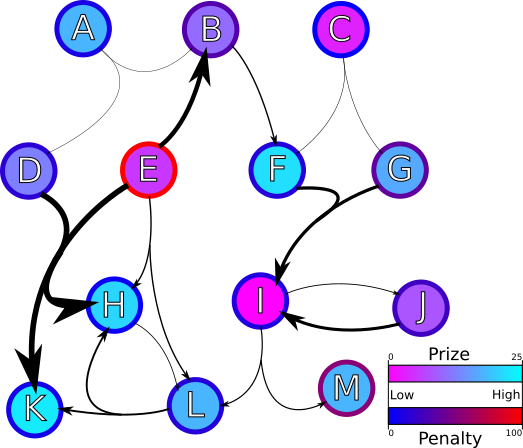
\includegraphics{example-hypergraph-weighted}
  \caption{The same hypergraph as in \ref{fig:example-hypergraph}, now weighted with node prizes (inner color) and dangling penalties (outer color). Edge thickness corresponds with edge weight. Intuitively, to find the PCSHT for this hypergraph, we want to find the subnetwork that maximizes the amount of blue, and minimizes the amount of both red nodes and thick lines.}
  \label{fig:example-hypergraph-weighted}
  \end{center}
\end{figure}

\section{Hyperpaths \& Connectivity}
In order to find the shortest route between two vertices, in a directed hypergraph, we define the notion of a \textit{hyperpath}, $P$, on the directed hypergraph $\mathcal{H}$.  We think of $P(s,t)$ as the list of vertices and hyperedges that one must pass through in order to traverse through the directed hypergraph from vertex $s$ to $t$. The existence of a hyperpath between two nodes encodes the notion of ``connectivity" between those nodes.  If a hyperpath exists between nodes $s$ and $t$, we say that they are \textit{connected}. Furthermore, given some root hypernode, $u$, we refer to the set of all nodes, $V$ in a hypergraph for which there exists some $P(u,v)$ (where $v \in V$) as a \textit{hypertree}. This is a useful definition, because it allows us the notion of a \textit{connected hypergraph}, a hypergraph in which every node is connected by some hyperpath to every other node in the hypergraph.\par

\subsection{Directed Hyperpaths}

There are many ways in which we can define hyperpaths, but for the purposes of finding Steiner Trees in directed hypergraphs, we must define a simple \textit{directed hyperpath} between nodes $s$ and $t$. We can think of a directed hyperpath $P(s,t)=\{s,e_2,v_3,...,e_{n-1},t\}$ as an ordered list of nodes and edges, beginning with $s$ and ending with $t$ such that for any edge, $e_i$, in the path, $v_{i-1}$ is in the tail of $e_i$, and $v_{i+1}$ is in the head of $e_i$.\par

\section{Definition of PCSHT}

We now can define the Prize-Collecting Steiner Hypertree (PCSHT), $\mathcal{S} = (V^\prime,E^\prime)$, to be the set of hypernodes and hyperedges for which total vertex prizes are maximized, and total edge weights (and dangling penalties) are minimized.  The Steiner Hypertree produced should satisfy the following properties:

\begin{itemize}
  \item{There should be no simple cycles between nodes in $\mathcal{S}$.}
  \item{The value of all prizes included in $\mathcal{S}$ should be maximal.}
  \item{The solution should minimal with respect to edges. \textit{(Should this be defined?)}}
  \item{The solution should consist of one or more parallel subnetworks. \textit{(Define this in the HYPERPATHS AND CONNECTIVITY section)}}
  \item{If an edge is included in the solution, every hypernode that is incident on that edge should also be included.}
\end{itemize}

In addition to these properties, it is also necessary for us to define two classes of nodes that may be present in a PCSHT: danging nodes and chads (\textit{names subject to change}).  We say a node is \textit{dangling} if it is present in a PCSHT and does not have any incoming hyperedge in the PCSHT (that is, it is not in the tail of any edge in the hypergraph). We can define a dangling node, $d$ as any node such $d \in V^\prime$ and $d \notin T(e)$ for all $e \in \mathcal{S}$. Similarly, we say a node is a \textit{chad} if it is present in a PCSHT, and not in the head of any edge in the hypergraph. A chad, $c$, is defined as any node $c \in V^\prime$ and $c \notin T(e)$ for all $e \in \mathcal{S}$.\par

\textit{PUT IN AN IMAGE SHOWING DANGLERS AND CHADS}

\chapter{Formulation of ILP}

In order for us define and develop a Prize-Collecting Steiner Hyptertree, we begin by formulating the notion of a \textit{Steiner Hypertree}. This allows us to develop an implementation that where some nodes, referred to as our \textit{target set}, are included in the solution, by definition. We begin like this to make the development and debugging of the ILP slightly easier, since it allows us to work from the target set to other nearby nodes, instead of forcing the ILP to discover every node that it needs to include.\par
To make our Steiner Hypertree, $\mathcal{S}$, we begin with a ``parent" hypergraph, $\mathcal{H} = (V,E)$, and a set of target nodes, $T$, such that $T \subseteq V$.  We refer to each hypernode as some $x$ such that $x \in V$\footnote{We use ``$x$" as an element of $V$, rather than lowercase ``$v$" to avoid the visual confusion between lowercase $v$ and uppercase $V$ (REMOVE THIS IF CHANGING TO V'S LOOKS OKAY)}, and each edge is some $e$ such that $e \in E$.  When building $\mathcal{H}$, we initially seed the hypergraph.  Each hyperedge is assigned a weight, that is, a cost associated with including that edge in the solution hypergraph, $\mathcal{S}$.  We then assign each hypernode in $\mathcal{H}$ two values, a prize for being included in $\mathcal{S}$, as well as a penalty associated with being a \textit{dangling} hypernode.\par



% \begin{itemize}
% 	\item The prizes for vertices included in $\mathcal{S}$ should be maximized.
% 	\item The costs for edges included in $\mathcal{S}$ should be minimized.
% 	\item All members of $T$ are included in $\mathcal{S}$.
% 	\item Each vertex that is incident (included in either the head or the tail) on an edge included in $\mathcal{S}$ is also in $\mathcal{S}$.
% 	\item All vertices included in $\mathcal{S}$ satisfy one of two conditions:
% 	\begin{itemize}
% 		\item The vertex has at least one incoming hyperedge that is also in $\mathcal{S}$.
% 		\item The vertex is dangling.
% 	\end{itemize}
% 	\item Hanging penalties for dangling nodes included in $\mathcal{S}$ are minimized.
% \end{itemize}
%
% \begin{figure}[thbp]
%   \begin{center}
%     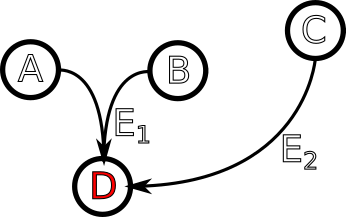
\includegraphics{dummy-before}
%   \caption{A simple hypergraph.}
%   \label{fig:dummy-before}
%   \end{center}
% \end{figure}

\section{Steiner Hypertree ILP}

To solve for solutions to the Prize Collecting Steiner Tree

Given an input hypergraph $\mathcal{H}=(V,E)$, and a set of target nodes, $T$, we construct a Steiner Hypertree, (DEFINE) $\mathcal{S}= (V^\prime,E^\prime)$, where $V^\prime \subseteq V$ and $E^\prime \subseteq E$.  We build $\mathcal{S}$ using an ILP which encodes the definition of a Steiner Hypertree.  In order to accomplish this, we define three indicator variables, $\alpha_v$, $\alpha_e$, and $\delta_v$, where $v$ and $e$ are hypernodes or hyperedges in $\mathcal{H}$.  If hypernode $x$ is in the solution of the ILP, $\alpha_v$ will have a value of 1, otherwise it will be equal to 0.  Similarly, if edge $e$ is present in the solution, $\alpha_e$ will take a value of 1. The value of $\delta_v$ will be determined by whether a hypernode is dangling.\par

We find the Steiner Hypergraph $\mathcal{S}$ by optimizing the function:

\begin{equation} \label{eq:ilpsum}
 \argmax_{\alpha, \delta} \sum_{v \in V} g_v \alpha_v - \sum_{e \in E} c_e \alpha_e - \sum_{v \in V} h_v \delta_v
\end{equation}

Subject to the set of linear constraints (\emph{Would it be a good idea to change these so that they all use $\leq$, rather than a mix of $\leq$ and $\geq$?}):

\begin{align}
 \alpha_v \geq 1 \qquad\qquad &\forall\; v \in T\label{eq:ilpT}\\
 \sum_{v \in H(e)} \alpha_v \geq \lvert H(e)\rvert \alpha_e \qquad\qquad &\forall\; e \in E\label{eq:ilpinchead}\\
 \sum_{v \in T(e)} \alpha_v \geq \lvert T(e)\rvert \alpha_e\qquad\qquad &\forall\; e \in E\label{eq:ilpinctail}\\
 \delta_v \leq \alpha_v \qquad\qquad &\forall\; v \in V\label{eq:ilpdang1}\\
 \delta_v \geq \alpha_{v} - \sum_{e:v \in H(e)} \alpha_e \qquad\qquad &\forall\; v \in V\label{eq:ilpdang2}\\
0 \leq \delta_v \leq 1 \qquad\qquad &\forall\; v \in V\label{eq:ilpdang3}%
\end{align}%


Here, the objective function \eqref{eq:ilpsum} tries combinations of nodes ($\alpha_v$), edges ($\alpha_e$), and dangling nodes ($\delta_v$) that maximize the sums of node prizes ($g_v$), minimize the sums of edge costs ($c_e$), and minimize the sums of dangling penalties ($h_v$). Constraint \eqref{eq:ilpT} encodes that every target node in $T$ is in the solution, $\mathcal{S}$.  Constraints \eqref{eq:ilpinchead} and \eqref{eq:ilpinctail} ensure that if an edge is in $\mathcal{S}$, any nodes incident on that edge (i.e. in the head or tail of that edge) will also be in $\mathcal{S}$.  Finally, constraints \eqref{eq:ilpdang1}, \eqref{eq:ilpdang2}, and \eqref{eq:ilpdang3} encode the ability for nodes to dangle if they do not have an incoming edge.\par

\begin{figure}[!htbp]
  \begin{minipage}[b]{0.60\linewidth}
    \centering
    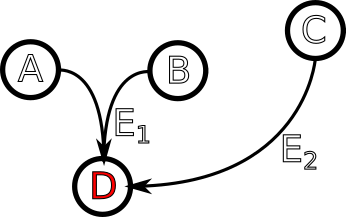
\includegraphics{dummy-before}
    \par\vspace{0pt}
  \end{minipage}%
  \begin{minipage}[b]{0.30\linewidth}
    \centering%
    \begin{tabular}{ |l|l|l| }%
      \hline%
      \multicolumn{3}{|c|}{Nodes} \\%
      \hline \hline
      Node & $g_v$ &  $h_v$ \\ \hline%
      A & 10 &  1\\ \hline%
      B & 10 &  1\\ \hline%
      C & 1 &  10\\ \hline%
      D & 10 &  10\\ \hline%
    \end{tabular}%
    \par\vspace{0pt}
  \end{minipage}
  \begin{minipage}[b]{0.30\linewidth}
    \centering%
    \begin{tabular}{ |l|l| }%
      \hline%
      \multicolumn{2}{|c|}{Edges} \\%
      \hline \hline
      Edge & $c_e$ \\ \hline%
      $E_1$ & 1 \\ \hline%
      $E_2$ & 10 \\ \hline%
    \end{tabular}%
    \par\vspace{0pt}
  \end{minipage}
\caption{A simple hypergraph, and its associated node and edge weights. \emph{This obviously needs to be re-formatted to not look terrible.}}
\label{fig:dummy-before}
\end{figure}

\emph{Should I start a new subsection here?}\par

Consider the hypergraph shown in Figure \ref{fig:dummy-before}. For this hypergraph, the PCSHT that comes from this graph should consist of hypernodes $A$, $B$, and $D$, as well as hyperedge $E_1$. This is obvious, since nodes $A$ and $B$, which will be dangling in the solution, both have low dangling penalties and high prizes, while node $C$ has a very large dangling penalty relative to its prize. Similarly, $E_1$ has a relatively low cost, whereas $E_2$ has a very high cost. Finally, $D$ is considered a target, in this case, and is therefore automatically included in the solution. Knowing what the solution should be, we can use this hypergraph to demonstrate the effect of each linear constrain in our ILP.\par

We now know that, for the optimal PCSHT, $\alpha_A$, $\alpha_D$, $\alpha_D$, and $\alpha_{E_1}$ are all equal to 1 (that is, they are included in the solution), and $\alpha_C$ and $\alpha_{E_2}$ are equal 0. Additionally, we know that in this solution $A$ and $B$ are dangling nodes, therefore $\delta_A$ and $\delta_B$ are both 1, and $\delta_C$ and $\delta_D$ are both 0. Finally, we are given that $D$ is a target node, hence $T=\{D\}$.\par

First let us look at the objective function, Equation (\emph{not actually an equation. Does this matter?}) \eqref{eq:ilpsum}. We can call each of the three sums included the equation which calculate the total node prizes, edge costs, and dangling penalties $\Xi$, $\Phi$, and $\Psi$, respectively. Given the values of $\alpha_v$, $\alpha_e$, and $\delta_v$ that we know should yield the PCSHT, we get find:
\begin{gather*}
 \Xi = 30\\
 \Phi = 1\\
 \Psi = 2\\
 \implies \Xi - \Phi - \Psi = 27\\
\end{gather*}%
If $C$ or $E_2$ were to be added, or any node or edge were removed from the PCSHT, the total value of the objective function would decrease, therefore yielding a suboptimal solution to the ILP.\par

Now, we can begin to look at how each linear constraint governs the behavior of the ILP. Let's begin with constraint \eqref{eq:ilpT}. For our hypergraph, $T$ only has one element, $D$, constraint \eqref{eq:ilpT} only needs to be checked for one node. We know that $\alpha_D = 1$, therefore constraint \eqref{eq:ilpT} simplifies to:
\begin{align*}
  \alpha_D &\geq 1\\
  1 &\geq 1\\
\end{align*}
We see that constraint \eqref{eq:ilpT} holds for all $v$ in $T$, therefore we know that all members of the target set are included in the PCSHT.\par

Next, we can look at constraints \eqref{eq:ilpinchead} and \eqref{eq:ilpinctail}. Since these constraints are the same, except for whether they are concerned with the head or tail of a hyperedge, we can evaluate the effect of just constraint \eqref{eq:ilpinchead}, and assume that constraint \eqref{eq:ilpinctail} works in the same way (\emph{Is this an okay assumption? Should I change it to look at the tails since there is a little more going on with those?}). To assess this constraint, we must see how if the inequality holds for all edges in the hypergraph. We begin by looking at $E_1$. We know that $H({E_1})=D$, and that $\lvert H(e) \rvert = 1$, therefore we can check:
\begin{align*}
  \alpha_D &\geq 1 \times \alpha_{E_1}\\
  1 &\geq 1 \times 1\\
  1 &\geq 1\\
\end{align*}%
So, we see that constraint \eqref{eq:ilpinchead} holds for $E_1$. Now, we can check for $E_2$ (whose head is also only $D$):
\begin{align*}
  \alpha_D &\geq 1 \times \alpha{E_2}\\
  1 &\geq 1 \times 0\\
  1 &\geq 0\\
\end{align*}%
We see that this inequality also holds. This means that, since the inequality holds for all hyperedges, that for every edge in the hypergraph, its head is also included in the hypergraph. We can easily extend this to see that \eqref{eq:ilpinctail} enforces the same for the tails of every hyperedge.\par

Finally, we can look at the three constraints that allow hypernodes to be dangling: constraints \eqref{eq:ilpdang1}, \eqref{eq:ilpdang2}, and \eqref{eq:ilpdang3}. First, we look at constraint \eqref{eq:ilpdang1} \emph{I need to figure out the proper way to align these.}:
\begin{alignat*}{4}
  \delta_A &\leq \alpha_A \qquad \delta_B &&\leq \alpha_B \qquad \delta_C &&\leq \alpha_C \qquad \delta_D &&\leq \alpha_D\\
  1 &\leq 1 \qquad 1 &&\leq 1 \qquad 0 &&\leq 0 \qquad 0 &&\leq 1\\
\end{alignat*}
Now, we see that constraint \eqref{eq:ilpdang1} holds for all nodes in the PCSHT. \emph{I will get the other two constraints up soon.}\par

\section{Danglers and Chads Problem}

When we implement the ILP in a more complex hypergraph, such as the hypergraph shown in Figure \ref{fig:example-hypergraph-weighted}, we find that it creates a hypergraph that consists of multiple smaller hypergraphs (Figure \ref{fig:example-hypergraph-weighted-after-ILP}), rather than a continuous subnetwork. Our original implementatioin ends up returning a group of disconnected hypergraphs that represent regions with high prize to edge/dangling cost ratios, separated by gaps where they parent hypergraph had regions of low prize to edge/dangling cost ratios. While this result is intersting, in itself, it will not necessarily create a soltion that is biologically interesting, once we begin looking for PCSHTs in pathway signaling data.\par

To fix this problem, we must incorporate the notion of hyperpaths and connectedness to our implementation of the PCSHT.
\begin{figure}[thbp]
  \begin{center}
    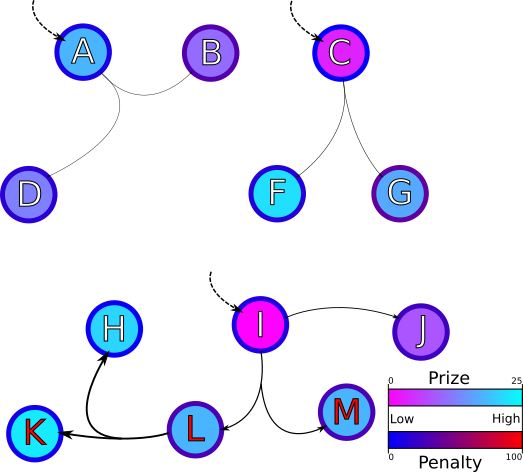
\includegraphics{example-hypergraph-weighted-after-ILP}
  \caption{The output of our ILP, when it is run on the hypergraph shown in Figure \ref{fig:example-hypergraph-weighted}. The dashed arrows indicate a dangling hypernode.}
  \label{fig:example-hypergraph-weighted-after-ILP}
  \end{center}
\end{figure}

\chapter{Implementation of PCSHT in PPI Data}

  \section{Network Construction \textit{HOW DO I REFERENCE HALP}}
  In order to construct directed signaling hypergraphs of biological pathways, we use pathway data from preexisting, curated protein-protein interaction networks, available publically. For this, pathway signaling information was downloaded from the curated Reactome pathway database (\cite{Croft2014}, \cite{Milacic2012}), and parsed into two flat files containing node and edge information necessary to construct the hypergraph (See Appendix B).\par
  The networks generated from the Reactome database specify each hypernode as a combination of one or more proteins or small molecules. For simplicity, each hypernode was ``converted" into a regular node for the purpose of algorithm implementation, and the components' information was saved so that they could be reconstructed \textit{post hoc}. Additionally, each hyperedge contained information about whether the reaction that it represented was regulated either positively or negatively by one or more nodes. Positive regulators were added to the tail of their respective hypernodes, since they are assumed to be necessary reactants for the edge, and should therefore be considered part of the signaling network. Negative regulators, on the other hand, were excluded from the flat files, since the way that they act on reactions poses poses an interesting problem in modeling, since the current definition of PCSHT assumes that all node prizes and edge weights are positive (see Future Directions).\par

  \section{Network Weighting}

    For the implementation PCSHT to create meaninful subnetworks, it is vital that the parent hypergraph have a meaningful, biologically informed weighting scheme applied.

    \subsection{Efficiency}


  \chapter{Efficacy (\& Proof??)}

  To assess the efficacy of this ILP in generating the correct Prize Collecting Steiner Hypertree, it is first necessary to perform a series of benchmarking tests on known datasets and hypergraphs.  This will allow us to determine if the algorithm is performing as expected, and generating results that can be corroborated manually.\par
%\section{References, Labels, Custom Commands and Footnotes}
%It is easy to refer to anything within your document using the \texttt{label} and \texttt{ref} tags.  Labels must be unique and shouldn't use any odd characters; generally sticking to letters and numbers (no spaces) should be fine. Put the label on whatever you want to refer to, and put the reference where you want the reference. \LaTeX\ will keep track of the chapter, section, and figure or table numbers for you.
%
%\subsection{References and Labels}
%Sometimes you'd like to refer to a table or figure, e.g. you can see in Figure \ref{subd2} that you can rotate figures . Start by labeling your figure or table with the label command (\verb=\label{labelvariable}=) below the caption (see the chapter on graphics and tables for examples). Then when you would like to refer to the table or figure, use the ref command (\verb=\ref{labelvariable}=). Make sure your label variables are unique; you can't have two elements named ``default." Also, since the reference command only puts the figure or table number, you will have to put  ``Table" or ``Figure" as appropriate, as seen in the following examples:
%
% As I showed in Table \ref{inheritance} many factors can be assumed to follow from inheritance. Also see the Figure \ref{subd} for an illustration.
%
%\subsection{Custom Commands}\label{commands}
%Are you sick of writing the same complex equation or phrase over and over?
%
%The custom commands should be placed in the preamble, or at least prior to the first usage of the command. The structure of the \verb=\newcommand= consists of the name of the new command in curly braces, the number of arguments to be made in square brackets and then, inside a new set of curly braces, the command(s) that make up the new command. The whole thing is sandwiched inside a larger set of curly braces.
%
%% Note: you cannot use numbers in your commands!
%\newcommand{\hydro}{H$_2$SO$_4$}
%
%In other words, if you want to make a shorthand for H$_2$SO$_4$, which doesn't include an argument, you would write: \verb=\newcommand{\hydro}{H$_2$SO$_4$}= and then when you needed  to use the command you would type \verb=\hydro=. (sans verb and the equals sign brackets, if you're looking at the .tex version). For example: \hydro
%
%\subsection{Footnotes and Endnotes}
%	You might want to footnote something.\footnote{footnote text} Be sure to leave no spaces between the word immediately preceding the footnote command and the command itself. The footnote will be in a smaller font and placed appropriately. Endnotes work in much the same way. More information can be found about both on the CUS site.
%
%\section{Bibliographies}
%	Of course you will need to cite things, and you will probably accumulate an armful of sources. This is why BibTeX was created. For more information about BibTeX and bibliographies, see our CUS site (\url{web.reed.edu/cis/help/latex/index.html})\footnote{\cite{reedweb:2007}}. There are three pages on this topic: {\it bibtex} (which talks about using BibTeX, at \url{/latex/bibtex.html}), {\it bibtexstyles} (about how to find and use the bibliography style that best suits your needs, at \url{/latex/bibtexstyles.html}) and {\it bibman} (which covers how to make and maintain a bibliography by hand, without BibTeX, at at \url{/latex/bibman.html}). The last page will not be useful unless you have only a few sources. There used to be APA stuff here, but we don't need it since I've fixed this with my apa-good natbib style file.
%
%\subsection{Tips for Bibliographies}
%\begin{enumerate}
%\item Like with thesis formatting, the sooner you start compiling your bibliography for something as large as thesis, the better. Typing in source after source is mind-numbing enough; do you really want to do it for hours on end in late April? Think of it as procrastination.
%\item The cite key (a citation's label) needs to be unique from the other entries.
%\item When you have more than one author or editor, you need to separate each author's name by the word ``and'' e.g.\\ \verb+Author = {Noble, Sam and Youngberg, Jessica},+.
%\item Bibliographies made using BibTeX (whether manually or using a manager) accept LaTeX markup, so you can italicize and add symbols as necessary.
%\item To force capitalization in an article title or where all lowercase is generally used, bracket the capital letter in curly braces.
%\item You can add a Reed Thesis citation\footnote{\cite{noble:2002}} option. The best way to do this is to use the phdthesis type of citation, and use the optional ``type'' field to enter ``Reed thesis'' or ``Undergraduate thesis''. Here's a test of Chicago, showing the second cite in a row\footnote{\cite{noble:2002}} being different. Also the second time not in a row\footnote{\cite{reedweb:2007}} should be different. Of course in other styles they'll all look the same.
%\end{enumerate}
%\section{Anything else?}
%If you'd like to see examples of other things in this template, please contact CUS (email cus@reed.edu) with your suggestions. We love to see people using \LaTeX\ for their theses, and are happy to help.
%
%
%\chapter{Mathematics and Science}
%\section{Math}
%	\TeX\ is the best way to typeset mathematics. Donald Knuth designed \TeX\ when he got frustrated at how long it was taking the typesetters to finish his book, which contained a lot of mathematics.
%
%	If you are doing a thesis that will involve lots of math, you will want to read the following section which has been commented out. If you're not going to use math, skip over this next big red section. (It's red in the .tex file but does not show up in the .pdf.)
%%
%%% MATH and PHYSICS majors: Uncomment the following section
%%
%$$\sum_{j=1}^n (\delta\theta_j)^2 \leq {{\beta_i^2}\over{\delta_i^2 + \rho_i^2}}
%\left[ 2\rho_i^2 + {\delta_i^2\beta_i^2\over{\delta_i^2 + \rho_i^2}} \right] \equiv \omega_i^2
%$$
%
%From Informational Dynamics, we have the following (Dave Braden):
%
%After {\it n} such encounters the posterior density for $\theta$ is
%
%$$
%\pi(\theta|X_1< y_1,\dots,X_n<y_n) \varpropto \pi(\theta) \prod_{i=1}^n\int_{-\infty}^{y_i}
%   \exp\left(-{(x-\theta)^2\over{2\sigma^2}}\right)\ dx
%$$
%
%
%
%Another equation:
%
%$$\det\left|\,\begin{matrix}%
%c_0&c_1\hfill&c_2\hfill&\ldots&c_n\hfill\cr
%c_1&c_2\hfill&c_3\hfill&\ldots&c_{n+1}\hfill\cr
%c_2&c_3\hfill&c_4\hfill&\ldots&c_{n+2}\hfill\cr
%\,\vdots\hfill&\,\vdots\hfill&
%  \,\vdots\hfill&&\,\vdots\hfill\cr
%c_n&c_{n+1}\hfill&c_{n+2}\hfill&\ldots&c_{2n}\hfill\cr
%\end{matrix}\right|>0$$
%
%%
%Lapidus and Pindar, Numerical Solution of Partial Differential Equations in Science and
%Engineering.  Page 54
%
%$$
%\int_t\left\{\sum_{j=1}^3 T_j \left({d\phi_j\over dt}+k\phi_j\right)-kT_e\right\}w_i(t)\ dt=0,
%   \qquad\quad i=1,2,3.
%$$
%
%L\&P  Galerkin method weighting functions.  Page 55
%
%$$
%\sum_{j=1}^3 T_j\int_0^1\left\{{d\phi_j\over dt} + k\phi_j\right\} \phi_i\ dt
%   = \int_{0}^1k\,T_e\phi_idt, \qquad i=1,2,3 $$
%
%Another L\&P (p145)
%
%$$
%\int_{-1}^1\!\int_{-1}^1\!\int_{-1}^1 f\big(\xi,\eta,\zeta\big)
%   = \sum_{k=1}^n\sum_{j=1}^n\sum_{i=1}^n w_i w_j w_k f\big( \xi,\eta,\zeta\big).
%$$
%
%Another L\&P (p126)
%
%$$
%\int_{A_e} (\,\cdot\,) dx dy = \int_{-1}^1\!\int_{-1}^1 (\,\cdot\,) \det[J] d\xi d\eta.
%$$
%
%
%\section{Physics}
%
%Many of the symbols you will need can be found on the math page (\url{http://web.reed.edu/cis/help/latex/math.html}) and the Comprehensive \LaTeX\ Symbol Guide (enclosed in this template download).  You may wish to create custom commands for commonly used symbols, phrases or equations, as described in Chapter \ref{commands}.
%
%\section{Biology}
%You will probably find the resources at \url{http://www.lecb.ncifcrf.gov/~toms/latex.html} helpful, particularly the links to bsts for various journals. You may also be interested in TeXShade for nucleotide typesetting (\url{http://homepages.uni-tuebingen.de/beitz/txe.html}).  Be sure to read the proceeding chapter on graphics and tables, and remember that the thesis template has versions of Ecology and Science bsts which support webpage citation formats.
%
%\chapter{Tables and Graphics}
%
%\section{Tables}
%	The following section contains examples of tables, most of which have been commented out for brevity. (They will show up in the .tex document in red, but not at all in the .pdf). For more help in constructing a table (or anything else in this document), please see the LaTeX pages on the CUS site.
%
%\begin{table}[htbp] % begins the table floating environment. This enables LaTeX to fit the table where it works best and lets you add a caption.
%\caption[Basic Table 1]{A Basic Table: Correlation of Factors between Parents and Child, Showing Inheritance}
%% The words in square brackets of the caption command end up in the Table of Tables. The words in curly braces are the caption directly over the table.
%\begin{center}
%% makes the table centered
%\begin{tabular}{c c c c}
%% the tabular environment is used to make the table itself. The {c c c c} specify that the table will have four columns and they will all be center-aligned. You can make the cell contents left aligned by replacing the Cs with Ls or right aligned by using Rs instead. Add more letters for more columns, and pipes (the vertical line above the backslash) for vertical lines. Another useful type of column is the p{width} column, which forces text to wrap within whatever width you specify e.g. p{1in}. Text will wrap badly in narrow columns though, so beware.
%\toprule % a horizontal line, slightly thicker than \hline, depends on the booktabs package
%  Factors &  Correlation between Parents \& Child & Inherited \\ % the first row of the table. Separate columns with ampersands and end the line with two backslashes. An environment begun in one cell will not carry over to adjacent rows.
%  \midrule % another horizontal line
%Education & -0.49 & Yes \\ % another row
%Socio-Economic Status & 0.28 & Slight \\
%Income & 0.08 & No\\
%Family Size & 0.19 & Slight \\
%Occupational Prestige &0.21 & Slight \\
%\bottomrule % yet another horizontal line
%\end{tabular}
%\end{center}
%\label{inheritance} % labels are useful when you have more than one table or figure in your document. See our online documentation for more on this.
%\end{table}
%
%	\clearpage
%%% \clearpage ends the page, and also dumps out all floats.
%%% Floats are things like tables and figures.
%
%If you want to make a table that is longer than a page, you will want to use the longtable environment. Uncomment the table below to see an example, or see our online documentation.
%
%	\begin{longtable}{||c|c|c|c||}
%	 	\caption[Long Table]{An example of a long table, with headers that repeat on each subsequent page: Results from the summers of 1998 and 1999 work at Reed College done
%by Grace Brannigan, Robert Holiday and Lien Ngo in 1998 and Kate Brown and
%Christina Inman in 1999.}\\ \hline
%	    	  \multicolumn{4}{||c||}{Chromium Hexacarbonyl} \\\hline
%		   State & Laser wavelength & Buffer gas & Ratio of $\frac{\textrm{Intensity
%at vapor pressure}}{\textrm{Intensity at 240 Torr}}$ \\ \hline
%		  \endfirsthead
%		\hline     State & Laser wavelength & Buffer gas & Ratio of
%$\frac{\textrm{Intensity at vapor pressure}}{\textrm{Intensity at 240 Torr}}$\\
%\hline
%		    \endhead
%
%	    $z^{7}P^{\circ}_{4}$ & 266 nm & Argon & 1.5 \\\hline
%	    $z^{7}P^{\circ}_{2}$ & 355 nm & Argon & 0.57 \\\hline
%	    $y^{7}P^{\circ}_{3}$ & 266 nm & Argon & 1 \\\hline
%	    $y^{7}P^{\circ}_{3}$ & 355 nm & Argon & 0.14 \\\hline
%	    $y^{7}P^{\circ}_{2}$ & 355 nm & Argon & 0.14 \\\hline
%	    $z^{5}P^{\circ}_{3}$ & 266 nm & Argon & 1.2 \\\hline
%	    $z^{5}P^{\circ}_{3}$ & 355 nm & Argon & 0.04 \\\hline
%	    $z^{5}P^{\circ}_{3}$ & 355 nm & Helium & 0.02 \\\hline
%	    $z^{5}P^{\circ}_{2}$ & 355 nm & Argon & 0.07 \\\hline
%	    $z^{5}P^{\circ}_{1}$ & 355 nm & Argon & 0.05 \\\hline
%	    $y^{5}P^{\circ}_{3}$ & 355 nm & Argon & 0.05, 0.4 \\\hline
%	    $y^{5}P^{\circ}_{3}$ & 355 nm & Helium & 0.25 \\\hline
%	    $z^{5}F^{\circ}_{4}$ & 266 nm & Argon & 1.4 \\\hline
%	    $z^{5}F^{\circ}_{4}$ & 355 nm & Argon & 0.29 \\\hline
%	    $z^{5}F^{\circ}_{4}$ & 355 nm & Helium & 1.02 \\\hline
%	    $z^{5}D^{\circ}_{4}$ & 355 nm & Argon & 0.3 \\\hline
%	    $z^{5}D^{\circ}_{4}$ & 355 nm & Helium & 0.65 \\\hline
%	    $y^{5}H^{\circ}_{7}$ & 266 nm & Argon & 0.17 \\\hline
%	    $y^{5}H^{\circ}_{7}$ & 355 nm & Argon & 0.13 \\\hline
%	    $y^{5}H^{\circ}_{7}$ & 355 nm & Helium & 0.11 \\\hline
%	    $a^{5}D_{3}$ & 266 nm & Argon & 0.71 \\\hline
%	    $a^{5}D_{2}$ & 266 nm & Argon & 0.77 \\\hline
%	    $a^{5}D_{2}$ & 355 nm & Argon & 0.63 \\\hline
%	    $a^{3}D_{3}$ & 355 nm & Argon & 0.05 \\\hline
%	    $a^{5}S_{2}$ & 266 nm & Argon & 2 \\\hline
%	    $a^{5}S_{2}$ & 355 nm & Argon & 1.5 \\\hline
%	    $a^{5}G_{6}$ & 355 nm & Argon & 0.91 \\\hline
%	    $a^{3}G_{4}$ & 355 nm & Argon & 0.08 \\\hline
%	    $e^{7}D_{5}$ & 355 nm & Helium & 3.5 \\\hline
%	    $e^{7}D_{3}$ & 355 nm & Helium & 3 \\\hline
%	    $f^{7}D_{5}$ & 355 nm & Helium & 0.25 \\\hline
%	    $f^{7}D_{5}$ & 355 nm & Argon & 0.25 \\\hline
%	    $f^{7}D_{4}$ & 355 nm & Argon & 0.2 \\\hline
%	    $f^{7}D_{4}$ & 355 nm & Helium & 0.3 \\\hline
%	    \multicolumn{4}{||c||}{Propyl-ACT} \\\hline
%%	    State & Laser wavelength & Buffer gas & Ratio of $\frac{\textrm{Intensity
%%at vapor pressure}}{\textrm{Intensity at 240 Torr}}$\\ \hline
%	    $z^{7}P^{\circ}_{4}$ & 355 nm & Argon & 1.5 \\\hline
%	    $z^{7}P^{\circ}_{3}$ & 355 nm & Argon & 1.5 \\\hline
%	    $z^{7}P^{\circ}_{2}$ & 355 nm & Argon & 1.25 \\\hline
%	    $z^{7}F^{\circ}_{5}$ & 355 nm & Argon & 2.85 \\\hline
%	    $y^{7}P^{\circ}_{4}$ & 355 nm & Argon & 0.07 \\\hline
%	    $y^{7}P^{\circ}_{3}$ & 355 nm & Argon & 0.06 \\\hline
%	    $z^{5}P^{\circ}_{3}$ & 355 nm & Argon & 0.12 \\\hline
%	    $z^{5}P^{\circ}_{2}$ & 355 nm & Argon & 0.13 \\\hline
%	    $z^{5}P^{\circ}_{1}$ & 355 nm & Argon & 0.14 \\\hline
%	    \multicolumn{4}{||c||}{Methyl-ACT} \\\hline
%%	    State & Laser wavelength & Buffer gas & Ratio of $\frac{\textrm{Intensity
%% at vapor pressure}}{\textrm{Intensity at 240 Torr}}$\\ \hline
%	    $z^{7}P^{\circ}_{4}$ & 355 nm & Argon & 1.6, 2.5 \\\hline
%	    $z^{7}P^{\circ}_{4}$ & 355 nm & Helium & 3 \\\hline
%	    $z^{7}P^{\circ}_{4}$ & 266 nm & Argon & 1.33 \\\hline
%	    $z^{7}P^{\circ}_{3}$ & 355 nm & Argon & 1.5 \\\hline
%	    $z^{7}P^{\circ}_{2}$ & 355 nm & Argon & 1.25, 1.3 \\\hline
%	    $z^{7}F^{\circ}_{5}$ & 355 nm & Argon & 3 \\\hline
%	    $y^{7}P^{\circ}_{4}$ & 355 nm & Argon & 0.07, 0.08 \\\hline
%	    $y^{7}P^{\circ}_{4}$ & 355 nm & Helium & 0.2 \\\hline
%	    $y^{7}P^{\circ}_{3}$ & 266 nm & Argon & 1.22 \\\hline
%	    $y^{7}P^{\circ}_{3}$ & 355 nm & Argon & 0.08 \\\hline
%	    $y^{7}P^{\circ}_{2}$ & 355 nm & Argon & 0.1 \\\hline
%	    $z^{5}P^{\circ}_{3}$ & 266 nm & Argon & 0.67 \\\hline
%	    $z^{5}P^{\circ}_{3}$ & 355 nm & Argon & 0.08, 0.17 \\\hline
%	    $z^{5}P^{\circ}_{3}$ & 355 nm & Helium & 0.12 \\\hline
%	    $z^{5}P^{\circ}_{2}$ & 355 nm & Argon & 0.13 \\\hline
%	    $z^{5}P^{\circ}_{1}$ & 355 nm & Argon & 0.09 \\\hline
%	    $y^{5}H^{\circ}_{7}$ & 355 nm & Argon & 0.06, 0.05 \\\hline
%	    $a^{5}D_{3}$ & 266 nm & Argon & 2.5 \\\hline
%	    $a^{5}D_{2}$ & 266 nm & Argon & 1.9 \\\hline
%	    $a^{5}D_{2}$ & 355 nm & Argon & 1.17 \\\hline
%	    $a^{5}S_{2}$ & 266 nm & Argon & 2.3 \\\hline
%	    $a^{5}S_{2}$ & 355 nm & Argon & 1.11 \\\hline
%	    $a^{5}G_{6}$ & 355 nm & Argon & 1.6 \\\hline
%	    $e^{7}D_{5}$ & 355 nm & Argon & 1 \\\hline
%
%		\end{longtable}
%
%
\chapter{Future Directions}
 \begin{itemize}
   \item{Heat mapping to weight hypergraphs (Random walks).}
   \item{Computation of individual or multiple subnetworks.}
 \end{itemize}
%    \section{Figures}
%
% 	If your thesis has a lot of figures, \LaTeX\ might behave better for you than that other word processor.  One thing that may be annoying is the way it handles ``floats'' like tables and figures. \LaTeX\ will try to find the best place to put your object based on the text around it and until you're really, truly done writing you should just leave it where it lies.   There are some optional arguments to the figure and table environments to specify where you want it to appear; see the comments in the first figure.
%
% 	If you need a graphic or tabular material to be part of the text, you can just put it inline. If you need it to appear in the list of figures or tables, it should be placed in the floating environment.
%
% 	To get a figure from StatView, JMP, SPSS or other statistics program into a figure, you can print to pdf or save the image as a jpg or png. Precisely how you will do this depends on the program: you may need to copy-paste figures into Photoshop or other graphic program, then save in the appropriate format.
%
% 	Below we have put a few examples of figures. For more help using graphics and the float environment, see our online documentation.
%
% 	And this is how you add a figure with a graphic:
% 	\begin{figure}[h]
% 	% the options are h = here, t = top, b = bottom, p = page of figures.
% 	% you can add an exclamation mark to make it try harder, and multiple
% 	% options if you have an order of preference, e.g.
% 	% \begin{figure}[h!tbp]
%
% 	       \centering
% 	    % DO NOT ADD A FILENAME EXTENSION TO THE GRAPHIC FILE
% 	    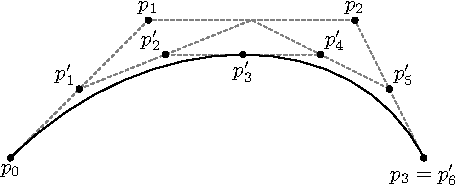
\includegraphics{subdivision}
% 	     \caption{A Figure}
% 	 \label{subd}
% 	\end{figure}
%
% \clearpage %% starts a new page and stops trying to place floats such as tables and figures
%
% \section{More Figure Stuff}
% You can also scale and rotate figures.
%  	\begin{figure}[h!]
%
% 	       \centering
% 	    % DO NOT ADD A FILENAME EXTENSION TO THE GRAPHIC FILE
% 	    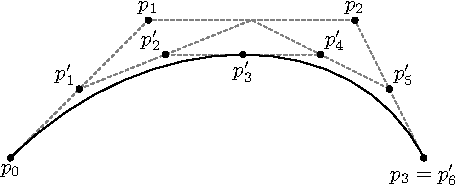
\includegraphics[scale=0.5,angle=180]{subdivision}
% 	    % if your figure shows up not where you want it, it may just be too big to fit. You can use the scale argument to shrink it, e.g. scale=0.85 is 85 percent of the original size.
% 	     \caption{A Smaller Figure, Flipped Upside Down}
% 	 \label{subd2}
% 	\end{figure}
%
% \section{Even More Figure Stuff}
% With some clever work you can crop a figure, which is handy if (for instance) your EPS or PDF is a little graphic on a whole sheet of paper. The viewport arguments are the lower-left and upper-right coordinates for the area you want to crop.
%
%  	\begin{figure}[h!]
% 	    	       \centering
% 	    % DO NOT ADD A FILENAME EXTENSION TO THE GRAPHIC FILE
% 	   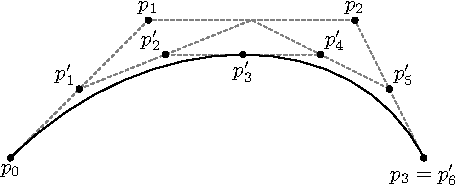
\includegraphics[clip=true, viewport=.0in .0in 1in 1in]{subdivision}
% 	    \caption{A Cropped Figure}
% 	 \label{subd3}
% 	\end{figure}
%
%       \subsection{Common Modifications}
%       The following figure features the more popular changes thesis students want to their figures. This information is also on the web at \url{web.reed.edu/cis/help/latex/graphics.html}.
%            \renewcommand{\thefigure}{0.\arabic{figure}} %Renumbers the figure to the type 0.x
%     \addtocounter{figure}{4} %starts the figure numbering at 4
%     \begin{figure}[htbp]
%     \begin{center}
%    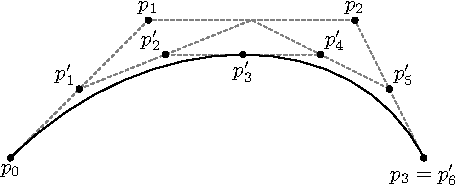
\includegraphics[scale=0.5]{subdivision}
%     \caption[Flower type and percent specialization]{\footnotesize{Interaction bar plot showing the degree of specialization for each flower type.}} %the special ToC caption is in square brackets. The \footnotesize makes the figure caption smaller
%     \label{barplot}
%     \end{center}
%     \end{figure}
%
\chapter*{Conclusion}
         \addcontentsline{toc}{chapter}{Conclusion}
	\chaptermark{Conclusion}
	\markboth{Conclusion}{Conclusion}
	\setcounter{chapter}{4}
	\setcounter{section}{0}

Here's a conclusion, demonstrating the use of all that manual incrementing and table of contents adding that has to happen if you use the starred form of the chapter command. The deal is, the chapter command in \LaTeX\ does a lot of things: it increments the chapter counter, it resets the section counter to zero, it puts the name of the chapter into the table of contents and the running headers, and probably some other stuff.

So, if you remove all that stuff because you don't like it to say ``Chapter 4: Conclusion'', then you have to manually add all the things \LaTeX\ would normally do for you. Maybe someday we'll write a new chapter macro that doesn't add ``Chapter X'' to the beginning of every chapter title.

\section{More info}
And here's some other random info: the first paragraph after a chapter title or section head \emph{shouldn't be} indented, because indents are to tell the reader that you're starting a new paragraph. Since that's obvious after a chapter or section title, proper typesetting doesn't add an indent there.


%If you feel it necessary to include an appendix, it goes here.
    \appendix
      \chapter{Algorithms \& Programs}
      \chapter{Benchmarking Graphs \& Supplemental Data}

        The constructor \verb|build_lp.py| builds a \texttt{.lp} file that can be optimized by the ILP solver CPLEX. The constructor takes the following files as arguments, as well as a column delimeter (default ``\texttt{;}") and a node delimeter (default ``\texttt{,}").

        Edge file (\texttt{ex-edges.txt}):\\
        \rule{\textwidth}{1pt}
        \verbatiminput{../examples/ex-edges.txt}
        \rule{\textwidth}{1pt}

        \newpage

        Node file (\texttt{ex-nodes.txt}):\\
        \rule{\textwidth}{1pt}
        \verbatiminput{../examples/ex-nodes.txt}
        \rule{\textwidth}{1pt}

      \chapter{Biological Data}


%This is where endnotes are supposed to go, if you have them.
%I have no idea how endnotes work with LaTeX.

  \backmatter % backmatter makes the index and bibliography appear properly in the t.o.c...

% if you're using bibtex, the next line forces every entry in the bibtex file to be included
% in your bibliography, regardless of whether or not you've cited it in the thesis.
    \nocite{*}

% Rename my bibliography to be called "Works Cited" and not "References" or ``Bibliography''
% \renewcommand{\bibname}{Works Cited}

%    \bibliographystyle{bsts/mla-good} % there are a variety of styles available;
%  \bibliographystyle{plainnat}
% replace ``plainnat'' with the style of choice. You can refer to files in the bsts or APA
% subfolder, e.g.
 \bibliographystyle{APA/apa-good} % or
 \bibliography{thesis}
 % Comment the above two lines and uncomment the next line to use biblatex-chicago.
 %\printbibliography[heading=bibintoc]

% Finally, an index would go here... but it is also optional.
\end{document}
